% TikZ bar chart showing performance by difficulty
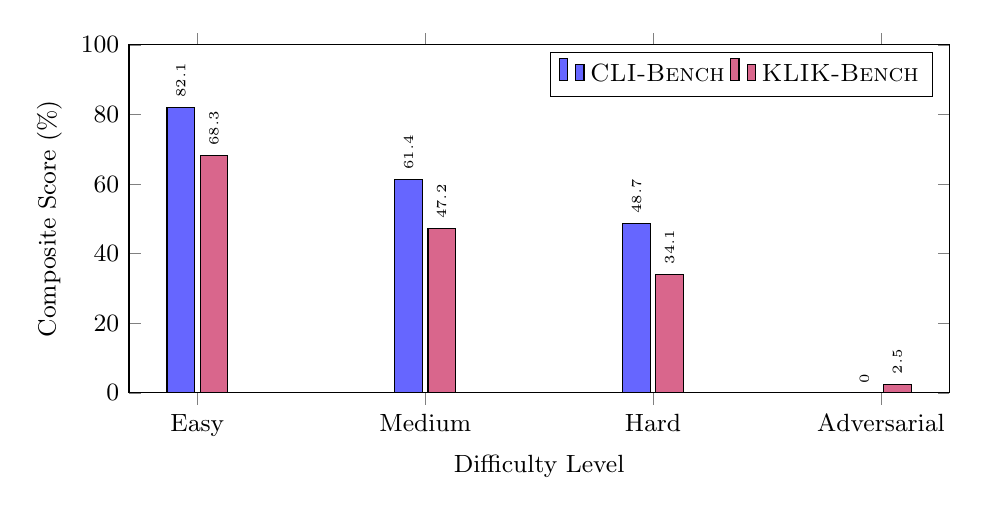
\begin{tikzpicture}
\begin{axis}[
    ybar,
    bar width=0.35cm,
    width=12cm,
    height=6cm,
    ylabel={Composite Score (\%)},
    ylabel style={font=\small},
    xlabel={Difficulty Level},
    xlabel style={font=\small},
    symbolic x coords={Easy, Medium, Hard, Adversarial},
    xtick=data,
    xticklabel style={font=\small},
    yticklabel style={font=\small},
    ymin=0,
    ymax=100,
    ytick={0,20,40,60,80,100},
    legend style={at={(0.98,0.98)}, anchor=north east, font=\small, legend columns=2},
    nodes near coords,
    nodes near coords style={font=\tiny},
    every node near coord/.append style={rotate=90, anchor=west},
]
% CLI-Bench data
\addplot[fill=blue!60] coordinates {(Easy, 82.1) (Medium, 61.4) (Hard, 48.7) (Adversarial, 0)};
% KLIK-Bench data
\addplot[fill=purple!60] coordinates {(Easy, 68.3) (Medium, 47.2) (Hard, 34.1) (Adversarial, 2.5)};
\legend{\textsc{CLI-Bench}, \textsc{KLIK-Bench}}
\end{axis}
\end{tikzpicture}
